%%%%%%%%%%%%%%%%%%%%%%%%%%%%%%%%%%%%%%%%%
% Beamer Presentation
% LaTeX Template
% Version 2.0 (March 8, 2022)
%
% This template originates from:
% https://www.LaTeXTemplates.com
%
% Author:
% Vel (vel@latextemplates.com)
%
% License:
% CC BY-NC-SA 4.0 (https://creativecommons.org/licenses/by-nc-sa/4.0/)
%
%%%%%%%%%%%%%%%%%%%%%%%%%%%%%%%%%%%%%%%%%

%----------------------------------------------------------------------------------------
%	PACKAGES AND OTHER DOCUMENT CONFIGURATIONS
%----------------------------------------------------------------------------------------

\documentclass[
	11pt, % Set the default font size, options include: 8pt, 9pt, 10pt, 11pt, 12pt, 14pt, 17pt, 20pt
	%t, % Uncomment to vertically align all slide content to the top of the slide, rather than the default centered
	%aspectratio=169, % Uncomment to set the aspect ratio to a 16:9 ratio which matches the aspect ratio of 1080p and 4K screens and projectors
]{beamer}


\usepackage{booktabs} % Allows the use of \toprule, \midrule and \bottomrule for better rules in tables
\usepackage{tikz}
\usepackage{colortbl}
\usepackage{array}
%----------------------------------------------------------------------------------------
%	SELECT LAYOUT THEME
%----------------------------------------------------------------------------------------

% Beamer comes with a number of default layout themes which change the colors and layouts of slides. Below is a list of all themes available, uncomment each in turn to see what they look like.

% \usetheme{default}
%\usetheme{AnnArbor}
%\usetheme{Antibes}
%\usetheme{Bergen}
% \usetheme{Berkeley}
%\usetheme{Berlin}
%\usetheme{Boadilla}
%\usetheme{CambridgeUS}
% \usetheme{Copenhagen}
%\usetheme{Darmstadt}
%\usetheme{Dresden}
%\usetheme{Frankfurt}
%\usetheme{Goettingen}
%\usetheme{Hannover}
%\usetheme{Ilmenau}
%\usetheme{JuanLesPins}
%\usetheme{Luebeck}
\usetheme{Madrid}
%\usetheme{Malmoe}
%\usetheme{Marburg}
%\usetheme{Montpellier}
% \usetheme{PaloAlto}
%\usetheme{Pittsburgh}
%\usetheme{Rochester}
% \usetheme{Singapore}
%\usetheme{Szeged}
%\usetheme{Warsaw}

%----------------------------------------------------------------------------------------
%	SELECT COLOR THEME
%----------------------------------------------------------------------------------------

% Beamer comes with a number of color themes that can be applied to any layout theme to change its colors. Uncomment each of these in turn to see how they change the colors of your selected layout theme.

% \usecolortheme{albatross}
%\usecolortheme{beaver}
%\usecolortheme{beetle}
%\usecolortheme{crane}
% \usecolortheme{dolphin}
%\usecolortheme{dove}
%\usecolortheme{fly}
%\usecolortheme{lily}
%\usecolortheme{monarca}
%\usecolortheme{seagull}
%\usecolortheme{seahorse}
%\usecolortheme{spruce}
%\usecolortheme{whale}
%\usecolortheme{wolverine}

%----------------------------------------------------------------------------------------
%	SELECT FONT THEME & FONTS
%----------------------------------------------------------------------------------------

% Beamer comes with several font themes to easily change the fonts used in various parts of the presentation. Review the comments beside each one to decide if you would like to use it. Note that additional options can be specified for several of these font themes, consult the beamer documentation for more information.

\usefonttheme{default} % Typeset using the default sans serif font
% \usefonttheme{serif} % Typeset using the default serif font (make sure a sans font isn't being set as the default font if you use this option!)
%\usefonttheme{structurebold} % Typeset important structure text (titles, headlines, footlines, sidebar, etc) in bold
%\usefonttheme{structureitalicserif} % Typeset important structure text (titles, headlines, footlines, sidebar, etc) in italic serif
%\usefonttheme{structuresmallcapsserif} % Typeset important structure text (titles, headlines, footlines, sidebar, etc) in small caps serif

%------------------------------------------------

%\usepackage{mathptmx} % Use the Times font for serif text
\usepackage{palatino} % Use the Palatino font for serif text

%\usepackage{helvet} % Use the Helvetica font for sans serif text
\usepackage[default]{opensans} % Use the Open Sans font for sans serif text
%\usepackage[default]{FiraSans} % Use the Fira Sans font for sans serif text
%\usepackage[default]{lato} % Use the Lato font for sans serif text

%----------------------------------------------------------------------------------------
%	SELECT INNER THEME
%----------------------------------------------------------------------------------------

% Inner themes change the styling of internal slide elements, for example: bullet points, blocks, bibliography entries, title pages, theorems, etc. Uncomment each theme in turn to see what changes it makes to your presentation.

\useinnertheme{default}
% \useinnertheme{circles}
% \useinnertheme{rectangles}
%\useinnertheme{rounded}
%\useinnertheme{inmargin}

%----------------------------------------------------------------------------------------
%	SELECT OUTER THEME
%----------------------------------------------------------------------------------------

% Outer themes change the overall layout of slides, such as: header and footer lines, sidebars and slide titles. Uncomment each theme in turn to see what changes it makes to your presentation.

\useoutertheme{default}
%\useoutertheme{infolines}
%\useoutertheme{miniframes}
%\useoutertheme{smoothbars}
%\useoutertheme{sidebar}
%\useoutertheme{split}
%\useoutertheme{shadow}
%\useoutertheme{tree}
%\useoutertheme{smoothtree}

%\setbeamertemplate{footline} % Uncomment this line to remove the footer line in all slides
%\setbeamertemplate{footline}[page number] % Uncomment this line to replace the footer line in all slides with a simple slide count

%\setbeamertemplate{navigation symbols}{} % Uncomment this line to remove the navigation symbols from the bottom of all slides

%----------------------------------------------------------------------------------------
%	PRESENTATION INFORMATION
%----------------------------------------------------------------------------------------

\title[Quantum Multi-string Matching]{Quantum Multi-string Matching} % The short title in the optional parameter appears at the bottom of every slide, the full title in the main parameter is only on the title page


\author[Allen Liu \and Kevin Tong]{Allen Liu \and Kevin Tong} % Presenter name(s), the optional parameter can contain a shortened version to appear on the bottom of every slide, while the main parameter will appear on the title slide

\institute[UW]{University of Waterloo} % Your institution, the optional parameter can be used for the institution shorthand and will appear on the bottom of every slide after author names, while the required parameter is used on the title slide and can include your email address or additional information on separate lines

\date[\today]{ECE 405C Winter 2025 \\ \today} % Presentation date or conference/meeting name, the optional parameter can contain a shortened version to appear on the bottom of every slide, while the required parameter value is output to the title slide

%----------------------------------------------------------------------------------------

\begin{document}

\newcommand*{\ket}[1]{\rvert#1\rangle}
%----------------------------------------------------------------------------------------
%	TITLE SLIDE
%----------------------------------------------------------------------------------------

\begin{frame}
    \titlepage % Output the title slide, automatically created using the text entered in the PRESENTATION INFORMATION block above
\end{frame}

%----------------------------------------------------------------------------------------
%	TABLE OF CONTENTS SLIDE
%----------------------------------------------------------------------------------------

% The table of contents outputs the sections and subsections that appear in your presentation, specified with the standard \section and \subsection commands. You may either display all sections and subsections on one slide with \tableofcontents, or display each section at a time on subsequent slides with \tableofcontents[pausesections]. The latter is useful if you want to step through each section and mention what you will discuss.

\begin{frame}
    \frametitle{Presentation Overview} % Slide title, remove this command for no title

    \tableofcontents % Output the table of contents (all sections on one slide)
    %\tableofcontents[pausesections] % Output the table of contents (break sections up across separate slides)
\end{frame}

%----------------------------------------------------------------------------------------
%	PRESENTATION BODY SLIDES
%----------------------------------------------------------------------------------------

\section{Problem Definition} % Sections are added in order to organize your presentation into discrete blocks, all sections and subsections are automatically output to the table of contents as an overview of the talk but NOT output in the presentation as separate slides

%------------------------------------------------


\begin{frame}
    \frametitle{String Matching}
    \begin{itemize}
        \item Text $S[0...n-1]$
        \item Pattern (or key) $P[0...m-1]$
        \item Strings from alphabet $\Sigma$
        \item Find set of indices $i$ such that $S[i..i+m] = P$
    \end{itemize}
    Example:
    \begin{itemize}
        \item $T$ = \texttt{"GTAT GATC TC"} (ignore spaces)
        \item $P_1$ = \texttt{"ATCT"}
        \item $P_2$ = \texttt{"TGAT"}
        \item $P_3$ = \texttt{"ACCC"}
        \item $P_1$ matches at 5, $P_2$ matches at 3, $P_3$ has no matches
    \end{itemize}
    \bigskip
    \begin{itemize}
        \item Multi-string matching: search $P_1, P_2, ...$ in $S$ simultaneously
    \end{itemize}
\end{frame}

%------------------------------------------------

\section{Classical Algorithms}
\subsection{Existing Algorithms}
\begin{frame}
    \frametitle{Classical Algorithms}
    \begin{itemize}
        \item Brute Force $\longrightarrow$ $O(mn)$
        \item Boyer-Moore $\longrightarrow$ $O(n+m)$, $O(mn)$ worst case
        \item Knuth-Morris-Pratt $\longrightarrow$ $O(n+m)$ worst case
        \item Suffix Tree/Array $\longrightarrow$ $O(m)/O(n\log n)$ + preproc
        \item Karp-Rabin - rolling hash $\longrightarrow$ $O(n+m)$ expected
    \end{itemize}

    \begin{center}

        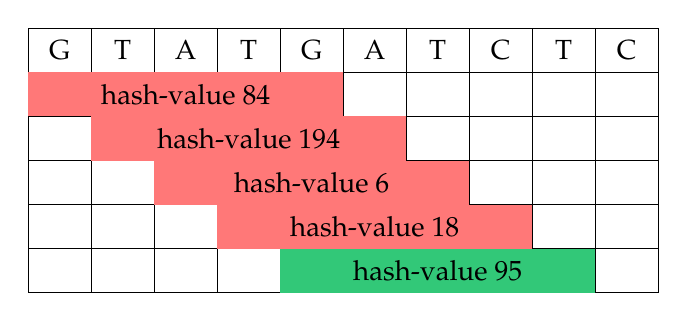
\begin{tikzpicture}[scale=0.8, y=0.7cm] % Scaling down the entire diagram with flatter cells
            % Define colors
            \definecolor{darkred}{RGB}{255,120,120}
            \definecolor{green}{RGB}{50,200,120}

            % Grid for cells with 6 rows
            \draw (0,0) -- (10,0);
            \draw (0,1) -- (10,1);
            \draw (0,2) -- (10,2);
            \draw (0,3) -- (10,3);
            \draw (0,4) -- (10,4);
            \draw (0,5) -- (10,5);
            \draw (0,6) -- (10,6);
            \draw (0,0) -- (0,6);
            \draw (1,0) -- (1,6);
            \draw (2,0) -- (2,6);
            \draw (3,0) -- (3,6);
            \draw (4,0) -- (4,6);
            \draw (5,0) -- (5,6);
            \draw (6,0) -- (6,6);
            \draw (7,0) -- (7,6);
            \draw (8,0) -- (8,6);
            \draw (9,0) -- (9,6);
            \draw (10,0) -- (10,6);

            % Add the letters at the top WITHOUT borders
            \foreach \x/\num in {0.5/G, 1.5/T, 2.5/A, 3.5/T, 4.5/G, 5.5/A, 6.5/T, 7.5/C, 8.5/T, 9.5/C} {
                    \node at (\x,5.5) {\num};
                }

            % Fill colors for different cells - one per row
            \fill[darkred] (0,4) rectangle (5,5); % First hash value
            \fill[darkred] (1,3) rectangle (6,4); % Second hash value 
            \fill[darkred] (2,2) rectangle (7,3); % Third hash value
            \fill[darkred] (3,1) rectangle (8,2); % Fourth hash value
            \fill[green] (4,0) rectangle (9,1); % Fifth hash value

            % Add the hash-value text
            \node at (2.5,4.5) {hash-value 84};
            \node at (3.5,3.5) {hash-value 194};
            \node at (4.5,2.5) {hash-value 6};
            \node at (5.5,1.5) {hash-value 18};
            \node at (6.5,0.5) {hash-value 95};

        \end{tikzpicture}

    \end{center}

    \begin{itemize}
        \item \alert{Polynomial Matching} $\longrightarrow$ $O(n\log n)$
    \end{itemize}
\end{frame}


%------------------------------------------------

\subsection{Polynomial Matching}
\begin{frame}
    \frametitle{Polynomial Matching}
    Calculate a fingerprint for $P$ and every $m$ character sequence in $S$; \alert {matching fingerprints} suggest pattern match!
    \bigskip
    \begin{align*}
        A & \mapsto -3 \\
        C & \mapsto 5  \\
        G & \mapsto -7 \\
        T & \mapsto 11
    \end{align*}
    \begin{align*}
        \texttt{"ATCT"}         & \longrightarrow 11x^3 + 5x^2 + 11x - 3                             \\
        \texttt{"GTAT GATC TC"} & \longrightarrow -7x^{15} + 11x^{14} - 3x^{13} + ... + 11x^7 + 5x^6
    \end{align*}
    Note that $P$ encoding is reversed (similar to convolution)
\end{frame}

%------------------------------------------------

\begin{frame}
    \frametitle{Polynomial Matching}
    Given polynomials
    \[
        P(x) = \sum_{i=0}^{m} a_i x^i, S(x) = \sum_{j=0}^{n} b_j x^j
    \]
    then
    \[
        R(x) = \sum_{k=0}^{m+n} c_k x^k
    \]
    where
    \[
        c_k = \sum_{i=0}^{k} a_i b_{k-i}, \quad \text{for } 0 \leq k \leq m+n,
    \]
    with the convention that \( a_i = 0 \) for \( i > m \) and \( b_j = 0 \) for \( j > n \).
\end{frame}

%------------------------------------------------

\begin{frame}
    \frametitle{Polynomial Matching}
    Coefficients of $R(x)$ correspond to ``dot products'' between substrings.
    \begin{align*}
        P(x) & = 11x^3 + 5x^2 + 11x - 3                                    \\
        S(x) & = -7x^{15} + 11x^{14} - 3x^{13} + ... + 11x^7 + 5x^6        \\
        R(x) & = ... + 71x^8 + 0x^9 + 276x^{10} + 98x^{11} - 4x^{12} + ...
    \end{align*}
    Degrees map to index:
    \begin{align*}
        15 & \text{ yields index } 0 \\
        14 & \text{ yields index } 1 \\
           & \hspace{0.8cm}...       \\
        11 & \text{ yields index } 4 \\
        10 & \text{ yields index } 5 \\
        9  & \text{ yields index } 6 \\
    \end{align*}
\end{frame}

%------------------------------------------------

\begin{frame}
    \frametitle{Polynomial Matching}
    Coefficients of $R(x)$ correspond to ``dot products'' between substrings.
    \begin{align*}
        P(x) & = 11x^3 + 5x^2 + 11x - 3                                    \\
        S(x) & = -7x^{15} + 11x^{14} - 3x^{13} + ... + 11x^7 + 5x^6        \\
        R(x) & = ... + 71x^8 + 0x^9 + 276x^{10} + 98x^{11} - 4x^{12} + ...
    \end{align*}
    Notice that $\|P\|^2 = 11^2 + 5^2 + 11^2 + (-3)^2 = 276$ \\
    \bigskip
    We get exact fingerprint match for single patterns. Let's extend to multiple patterns...
\end{frame}


%------------------------------------------------

\begin{frame}
    \frametitle{Polynomial Matching}
    Add patterns together:
    \begin{align*}
        P(x) & = P_1(x) + P_2(x)                                                        \\
        S(x) & = -7x^{15} + 11x^{14} - 3x^{13} + ... + 11x^7 + 5x^6                     \\
        R(x) & = ... + 94x^8 + 240x^9 + 272x^{10} + 64x^{11} + 296x^{12} - 60x^{13} ...
    \end{align*}
    \bigskip
    No more exact matches, but higher values = likelier index.
\end{frame}

%------------------------------------------------

\subsection{Polynomial Multiplication}
\begin{frame}
    \frametitle{Polynomial Multiplication}
    For two polynomials of degree $n$, 
    \begin{align*}
        A(x) &= a_0 + a_1x + a_2x^2 + \cdots + a_(n-1)x^{n-1} \\
        B(x) &= b_0 + b_1x + b_2x^2 + \cdots + b_(n-1)x^{n-1} \\ 
    \end{align*}
    The goal is to simply to find their product:
    \[
        C(x) = \sum_{j=0}^{n-1}\sum_{k=0}^{n-1}a_kb_kx^{j+k} 
    \]

    \begin{itemize}
        \item Naïve polynomial multiplication $\longrightarrow$ $O(n^2)$
        \item Karatsuba Algorithm $\longrightarrow$ $O(n^{\log_3 2}) = O(n^{1.59})$
        \item FFT $\longrightarrow$ $O(n\log n)$
    \end{itemize}

\end{frame}

%------------------------------------------------

\begin{frame}
    \frametitle{Polynomial Multiplication}
    For two polynomials of degree $n$, 
    \begin{align*}
        A(x) &= a_0 + a_1x + a_2x^2 + \cdots + a_(n-1)x^{n-1} \\
        B(x) &= b_0 + b_1x + b_2x^2 + \cdots + b_(n-1)x^{n-1} \\ 
    \end{align*}
    The goal is to simply to find their product:
    \[
        C(x) = \sum_{j=0}^{n-1}\sum_{k=0}^{n-1}a_kb_kx^{j+k} 
    \]
    The naïve approach is to directly evaluate the summation 
    (i.e. long multiplication/grade-school multiplication).
\end{frame}

%------------------------------------------------

\begin{frame}
    \frametitle{Efficient Polynomial Multiplication}
    Multiple algorithms for multiplication:
    \begin{itemize}
        \item Naïve polynomial multiplication $\longrightarrow$ $O(n^2)$
        \item Karatsuba Algorithm $\longrightarrow$ $O(n^{\log_3 2}) = O(n^{1.59})$
        \item FFT $\longrightarrow$ $O(n\log n)$
    \end{itemize}
\end{frame}

%------------------------------------------------

\begin{frame}
    \frametitle{Polynomial Multiplication with FFT}
    \begin{enumerate}
        \item Apply FFT to the coefficients of $A(x)$ and $B(x)$ \\
        With $\vec{a} = [a_0\,\,a_1\dots a_{n-1}]^T$ and $\vec{b} = [b_0\,\,b_1\dots b_{n-1}]^T$, then
        \begin{align*}
            \vec{\alpha} &= \text{FFT}(\vec{a}) \tag*{$O(n\log n)$} \\
            \vec{\beta} &= \text{FFT}(\vec{b}) \tag*{$O(n\log n)$}
        \end{align*}
        \item Perform the Hadamard (element-wise) product of coefficients
        \begin{align*}
            \vec{\gamma} &= \vec{\alpha} \odot \vec{\beta} \\
                &= [\alpha_0\beta_0\,\,\,\,\alpha_1\beta_1\dots\alpha_{n-1}\beta_{n-1}]^T \tag*{$O(n)$}
        \end{align*}
        \item Apply Inverse FFT
        \begin{align*}
            \vec{c} &= \text{IFFT}(\vec{\gamma}) \tag*{$O(n\log n)$}
        \end{align*}
    \end{enumerate}
\end{frame}

%------------------------------------------------

% \begin{frame}
%     \frametitle{Polynomial Multiplication with QFT}
%     \begin{enumerate}
%         \item Apply QFT to quantum states $\ket{\psi}$ and $\ket{\phi}$ 
%         that are amplitude encodings of polynomial cofficients \\
%         \item Perform the Hadamard (element-wise) product of 
%             $\text{QFT}(\ket{\psi})$ and $\text{QFT}(\ket{\phi})$
%         \item Apply Inverse QFT
%     \end{enumerate}
% \end{frame}

%------------------------------------------------

\section{Quantum Algorithms}
\subsection{Polynomial Multiplication with QFT}
\begin{frame}
    \frametitle{Polynomial Multiplication with QFT}
    \begin{center}
        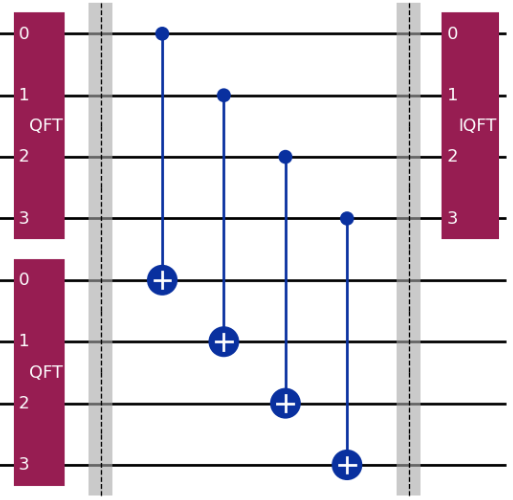
\includegraphics[scale=0.7]{basic_circuit.PNG}
    \end{center}
\end{frame}

%------------------------------------------------

\begin{frame}
    \frametitle{Using Measurement for Validity}
 To ensure the validity of quantum element-wise multiplication, 
    we require the last qubits to be measured as all zero.
    \newline\newline
    Consider the simplest case: the element-wise product of two qubits' states
    \begin{align*}
        &CNOT_{1\to 2}((a_0\ket{0} + a_1\ket{1}) \otimes (b_0\ket{0} + b_1\ket{1})) \\
        &= CNOT_{1\to 2}(a_0b_0\ket{00} + a_0b_1\ket{01} + a_1b_0\ket{10} + a_1b_1\ket{11}) \\
        &= a_0b_0\ket{00} + a_0b_1\ket{01} + a_1b_0\ket{11} + a_1b_1\ket{10} \\
    \end{align*}
    Note how the $a_0b_0$ and $a_1b_1$ products are only associated with terms where the second qubit is $\ket{0}$, 
    and a coefficient product can be ``chosen'' using the state of the first qubit.
\end{frame}

%------------------------------------------------

\begin{frame}
    \frametitle{Lists}
    \framesubtitle{Bullet Points and Numbered Lists} % Optional subtitle

    \begin{itemize}
        \item Lorem ipsum dolor sit amet, consectetur adipiscing elit
        \item Aliquam blandit faucibus nisi, sit amet dapibus enim tempus
              \begin{itemize}
                  \item Lorem ipsum dolor sit amet, consectetur adipiscing elit
                  \item Nam cursus est eget velit posuere pellentesque
              \end{itemize}
        \item Nulla commodo, erat quis gravida posuere, elit lacus lobortis est, quis porttitor odio mauris at libero
    \end{itemize}

    \bigskip % Vertical whitespace

    \begin{enumerate}
        \item Nam cursus est eget velit posuere pellentesque
        \item Vestibulum faucibus velit a augue condimentum quis convallis nulla gravida
    \end{enumerate}
\end{frame}

%------------------------------------------------


\begin{frame}
    \frametitle{Blocks of Highlighted Text}

    \begin{block}{Block Title}
        Lorem ipsum dolor sit amet, consectetur adipiscing elit. Integer lectus nisl, ultricies in feugiat rutrum, porttitor sit amet augue.
    \end{block}

    \begin{exampleblock}{Example Block Title}
        Aliquam ut tortor mauris. Sed volutpat ante purus, quis accumsan.
    \end{exampleblock}

    \begin{alertblock}{Alert Block Title}
        Pellentesque sed tellus purus. Class aptent taciti sociosqu ad litora torquent per conubia nostra, per inceptos himenaeos.
    \end{alertblock}

    \begin{block}{} % Block without title
        Suspendisse tincidunt sagittis gravida. Curabitur condimentum, enim sed venenatis rutrum, ipsum neque consectetur orci.
    \end{block}
\end{frame}

%------------------------------------------------


\begin{frame}
    \frametitle{Multiple Columns}
    \framesubtitle{Subtitle} % Optional subtitle

    \begin{columns}[c] % The "c" option specifies centered vertical alignment while the "t" option is used for top vertical alignment
        \begin{column}{0.45\textwidth} % Left column width
            \textbf{Heading}
            \begin{enumerate}
                \item Statement
                \item Explanation
                \item Example
            \end{enumerate}
        \end{column}
        \begin{column}{0.5\textwidth} % Right column width
            Lorem ipsum dolor sit amet, consectetur adipiscing elit. Integer lectus nisl, ultricies in feugiat rutrum, porttitor sit amet augue. Aliquam ut tortor mauris. Sed volutpat ante purus, quis accumsan dolor.
        \end{column}
    \end{columns}
\end{frame}

%------------------------------------------------



\begin{frame}
    \frametitle{Table}
    \framesubtitle{Subtitle} % Optional subtitle

    \begin{table}
        \begin{tabular}{l l l}
            \toprule
            \textbf{Treatments} & \textbf{Response 1} & \textbf{Response 2} \\
            \midrule
            Treatment 1         & 0.0003262           & 0.562               \\
            Treatment 2         & 0.0015681           & 0.910               \\
            Treatment 3         & 0.0009271           & 0.296               \\
            \bottomrule
        \end{tabular}
        \caption{Table caption}
    \end{table}
\end{frame}


%------------------------------------------------


\begin{frame}
    \frametitle{Definitions \& Examples}

    \begin{definition}
        A \alert{prime number} is a number that has exactly two divisors.
    \end{definition}

    \smallskip % Vertical whitespace

    \begin{example}
        \begin{itemize}
            \item 2 is prime (two divisors: 1 and 2).
            \item 3 is prime (two divisors: 1 and 3).
            \item 4 is not prime (\alert{three} divisors: 1, 2, and 4).
        \end{itemize}
    \end{example}

    \smallskip % Vertical whitespace

    You can also use the \texttt{theorem}, \texttt{lemma}, \texttt{proof} and \texttt{corollary} environments.
\end{frame}

%------------------------------------------------

\begin{frame}
    \frametitle{Theorem, Corollary \& Proof}

    \begin{theorem}[Mass--energy equivalence]
        $E = mc^2$
    \end{theorem}

    \begin{corollary}
        $x + y = y + x$
    \end{corollary}

    \begin{proof}
        $\omega + \phi = \epsilon$
    \end{proof}
\end{frame}

%------------------------------------------------

\begin{frame}
    \frametitle{Equation}

    \begin{equation}
        \cos^3 \theta =\frac{1}{4}\cos\theta+\frac{3}{4}\cos 3\theta
    \end{equation}
\end{frame}

%------------------------------------------------

\begin{frame}[fragile] % Need to use the fragile option when verbatim is used in the slide
    \frametitle{Verbatim}

    \begin{example}[Theorem Slide Code]
        \begin{verbatim}
			\begin{frame}
				\frametitle{Theorem}
				\begin{theorem}[Mass--energy equivalence]
					$E = mc^2$
				\end{theorem}
		\end{frame}\end{verbatim} % Must be on the same line
    \end{example}
\end{frame}

%------------------------------------------------

\begin{frame}
    Slide without title.
\end{frame}

%------------------------------------------------


\begin{frame}
    \frametitle{Citing References}

    An example of the \texttt{\textbackslash cite} command to cite within the presentation:

    \bigskip % Vertical whitespace

    This statement requires citation \cite{p1,p2}.
\end{frame}

%------------------------------------------------

\begin{frame} % Use [allowframebreaks] to allow automatic splitting across slides if the content is too long
    \frametitle{References}

    \begin{thebibliography}{99} % Beamer does not support BibTeX so references must be inserted manually as below, you may need to use multiple columns and/or reduce the font size further if you have many references
        \footnotesize % Reduce the font size in the bibliography

        \bibitem[Smith, 2022]{p1}
        John Smith (2022)
        \newblock Publication title
        \newblock \emph{Journal Name} 12(3), 45 -- 678.

        \bibitem[Kennedy, 2023]{p2}
        Annabelle Kennedy (2023)
        \newblock Publication title
        \newblock \emph{Journal Name} 12(3), 45 -- 678.
    \end{thebibliography}
\end{frame}

%----------------------------------------------------------------------------------------
%	ACKNOWLEDGMENTS SLIDE
%----------------------------------------------------------------------------------------

\begin{frame}
    \frametitle{Acknowledgements}

    \begin{columns}[t] % The "c" option specifies centered vertical alignment while the "t" option is used for top vertical alignment
        \begin{column}{0.45\textwidth} % Left column width
            \textbf{Smith Lab}
            \begin{itemize}
                \item Alice Smith
                \item Devon Brown
            \end{itemize}
            \textbf{Cook Lab}
            \begin{itemize}
                \item Margaret
                \item Jennifer
                \item Yuan
            \end{itemize}
        \end{column}
        \begin{column}{0.5\textwidth} % Right column width
            \textbf{Funding}
            \begin{itemize}
                \item British Royal Navy
                \item Norwegian Government
            \end{itemize}
        \end{column}
    \end{columns}
\end{frame}

%----------------------------------------------------------------------------------------
%	CLOSING SLIDE
%----------------------------------------------------------------------------------------

\begin{frame}[plain] % The optional argument 'plain' hides the headline and footline
    \begin{center}
        {\Huge The End}

        \bigskip\bigskip % Vertical whitespace

        {\LARGE Questions? Comments?}
    \end{center}
\end{frame}

%----------------------------------------------------------------------------------------

\end{document}